%% LyX 2.2.3 created this file.  For more info, see http://www.lyx.org/.
%% Do not edit unless you really know what you are doing.
\documentclass[english]{article}
\usepackage[T1]{fontenc}
\usepackage[latin9]{inputenc}
\usepackage{geometry}
\geometry{verbose,lmargin=2cm,rmargin=2cm}
\usepackage{babel}
\usepackage{float}
\usepackage{graphicx}
\usepackage[unicode=true,pdfusetitle,
 bookmarks=true,bookmarksnumbered=false,bookmarksopen=false,
 breaklinks=false,pdfborder={0 0 1},backref=false,colorlinks=false]
 {hyperref}
\usepackage{breakurl}

\makeatletter

%%%%%%%%%%%%%%%%%%%%%%%%%%%%%% LyX specific LaTeX commands.
%% Because html converters don't know tabularnewline
\providecommand{\tabularnewline}{\\}
\floatstyle{ruled}
\newfloat{algorithm}{tbp}{loa}
\providecommand{\algorithmname}{Algorithm}
\floatname{algorithm}{\protect\algorithmname}

\makeatother

\usepackage{listings}
\renewcommand{\lstlistingname}{Listing}

\begin{document}

\title{Classifying Books By Writing Style Using Machine Learning Techniques}

\author{By:\\
Or Hanoch, Devon Jarvis, Meir Rosendorff, Kimesha <insert indian last
name here>\\
Instructor:\\
Dr. Benjamin Rossman}

\maketitle
\setcounter{section}{-1}
\section{Introduction}

This project is part of the machine learning course held in the University
of the Witwatersrand and lectured by Dr. Benjamin Rossman. In this
project we use different machine learning techniques learnt in the
course to recognize which book, from a set of books, a given page
is from. In particular we were interested in doing this with the seven
Harry Potter books in order to see if there is any distinguishable
change in writing style as the series progressed.

We used the following techniques: Na�ve Bayes, k-means clustering,
and neural networks. The process and results are specified below.

\section{Na�ve Bayes}

\subsection{Background}

The Na�ve Bayes Algorithm uses a list of probabilities and Bayes Rule
to classify data into groups. 

\subsection{Methods}

\subsubsection{Data Processing }

We start off by splitting all the books into page sets (We will explain
later how we optimized the `pageSetSize` which is the number of pages
in a set). We then took around 20\% of these from each book and set
them aside for validation data which we used for training our hyperparameters,
we set a further 20\% aside for testing and the remaining 60\% we
used for training data. \\

We removed all punctuation from the data, except for question marks
and exclamation marks which were separated into their own words as
we felt this may give more insight as J.K. Rowling may have asked
more questions or written more exclamations in some books than others.\\

We then took our training data and we calculated the probability for
each word appearing in any one page set from each book. We did this
by counting the number of page sets a word appears in in each book
and dividing it by the total number of page sets in that book. This
gave us our probability tables, each of which contain probabilities
for around 20 000 words. Each of the tables contains a different number
of words because of how the data is split up and which data the trainer
sees and which is used for testing (see folder probTables where we
have stored each of our tables).Using the validation data we optimized
the hyperparameters `pageSetSize`, `upperThreshold`, `lowerThreshold`
and `requiredNum`. We did this using the following algorithm:

\begin{algorithm}
\caption{Keeping Relevant Words}

\begin{lstlisting}
for each pageSetSize ranging from 1  13:

	probailityTable = create probability table based off pageSetSize using trainingData
for each requiredNum in range 1 - 5

	currTable = probailityTable with words removed based off upperThreshold, lowerThreshold and requiredNum
	while accuracy on validation data is improving:

		while accuracy on validation data is improving:

			Decrease lowerThreshold by alpha
			currTable = probailityTable with words removed based off new upperThreshold, lowerThreshold and requiredNum
			Retest on validation data 

		while accuracy on validation data is improving:

			Increase upperThreshold by alpha
			currTable = probailityTable with words removed based off new upperThreshold, lowerThreshold and requiredNum
			Retest on validation data 

		Change alpha by a factor of a half
		If alpha is less than a threshold exit the loop

take the pageSetSize, upperThreshold, lowerThreshold and requiredNum that yield the best accuracy
test on testing data
\end{lstlisting}
\end{algorithm}

\subsubsection{Na�ve Bayes Procedure}

\subsubsection{Hyper-Perameter Tuning}

\subsection{Results}

The following graph shows the accuracy given for the different pageSetSizes
on our test data, it should be noted that since there are 7 options
a random guess will be correct 14.29\% of the time.

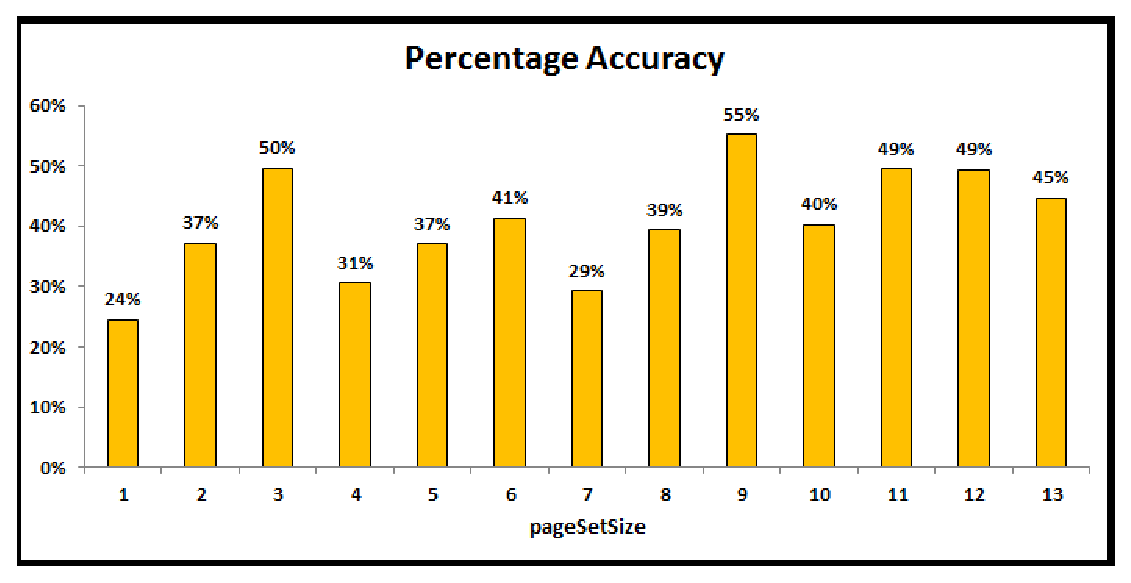
\includegraphics{naive_bayes/Images/percentageAccuracy}\\
It is quite clear a pageSetSize of 9 gives the highest accuracy of
55\%, we however feel that the pageSetSize of 3 pages with an accuracy
of 50\% is the best result as it balances as few pages as possible
with the best accuracy possible. In addition despite a pageSetSize
of 1 only having a 24\% accuracy this is nearly double random and
we feel it is still noteworthy and meaningful that based off a single
page we can classify with that accuracy.\\
It should also be noted that because we have a limited number of pages
(there are 4707 pages in the series) when we increase the pageSetSize
it decreases our dataset size. This means that the higher pageSetSizes
have less training data and less testing data so the results aren\textquoteright t
as trustworthy. We believe this is the reason that the percentage
accuracy doesn\textquoteright t change as drastically over the last
few pageSetSizes. The following table gives the breakup of pageSetSize
and dataset size.\\
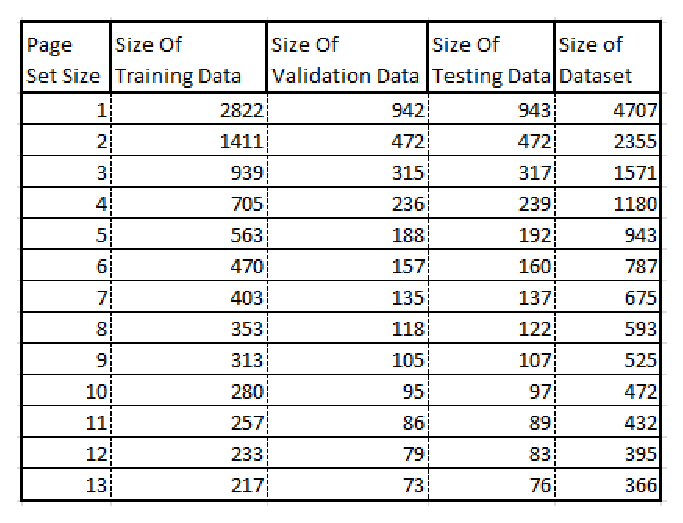
\includegraphics{naive_bayes/Images/pageSetSizeTable}\\
Thus the best classifier that we found was trained using the following
parameters: pageSetSize = 3 requiredNum = 2 upperThreshold = 7.05
\% lowerThreshold = 0.9 \% Trained on 939 pageSets Validated on 315
pageSets

\subsubsection{Confusion Matrix}

The following is the confusion matrix we got after testing this classifier
on 317 test cases

\begin{tabular}{|c|c|c|c|c|c|c|c|}
\hline 
 & 1 & 2 & 3 & 4 & 5 & 6 & 7\tabularnewline
\hline 
\hline 
1 &  &  &  &  &  &  & \tabularnewline
\hline 
2 &  &  &  &  &  &  & \tabularnewline
\hline 
3 &  &  &  &  &  &  & \tabularnewline
\hline 
4 &  &  &  &  &  &  & \tabularnewline
\hline 
5 &  &  &  &  &  &  & \tabularnewline
\hline 
6 &  &  &  &  &  &  & \tabularnewline
\hline 
7 &  &  &  &  &  &  & \tabularnewline
\hline 
\end{tabular}

This confusion matrix has an accuracy of 49.53\%. There a quite a
few interesting observations that can be made about the harry potter
books from this matrix. 

The first thing that jumps out as obvious in this matrix (and is reflected
in all the others) is an obvious bias to book 1 and book 5.

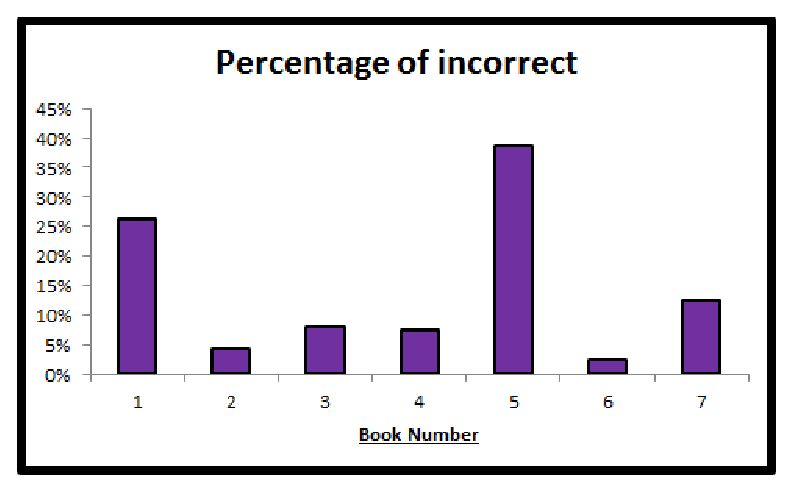
\includegraphics{naive_bayes/Images/inCorrectPerBook}

This could indicate multiple things. The bias towards book 1 is most
likely because a lot is most likely introduced in book one that is
referenced in later books. The bias towards book 5 could be because
book 5 is the largest of all the harry potter books. It could also
mean that in book 5 there are a lot of references and similarities
to all of the earlier books and for this reason they are easily confused
with book 5 and the classifier chooses book 5 over them since it is
nearly double the size of the earlier books and thus more likely.
See the following Table:

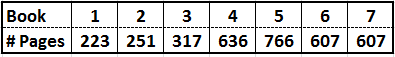
\includegraphics{naive_bayes/Images/numBookPages}

Another interesting aspect of this confusion matrix is that other
than the bias to book 5 it is nearly an upper triangular matrix, with
majority of the incorrect guesses being in the upper triangle. This
means that when it chooses incorrectly the classifier is more likely
to pick an earlier book than it is to pick a later one. This result
is to be expected as it means the later books are more similar to
the earlier books than the earlier books are to the later ones. This
is most likely because names of people and places, jargon and ideas
are introduced in one book and carried through to the later books
but all the books before the one in which this was introduced will
have no reference to it. This is not only evident in this matrix but
in all the other matrices as well, see the following graph which shows
the split up of incorrect guesses between those that where later than
the correct book and those that where earlier, as you can see majority
of the time we classify as an earlier book rather than a later book. 

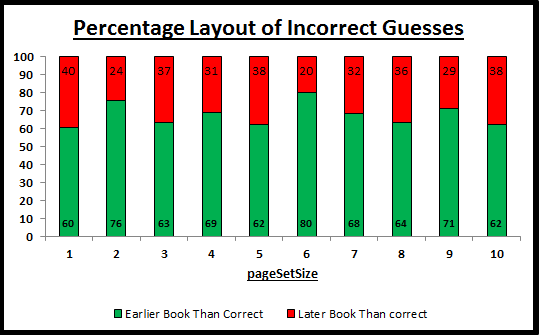
\includegraphics{naive_bayes/Images/incorrectLayout}

A further surprising idea seen from the confusion matrices is that
you would expect that when a page set is classified incorrectly it
is most likely to be classified as either the previous book or the
following book. The confusion matrices show that on average 29\% of
the incorrect guesses are classified as either the previous or following
book. This however is very close to random as the probability of a
page set being any one book is 14\%, so the probability of it being
any two is 28\%, thus not much information can be derived from this.

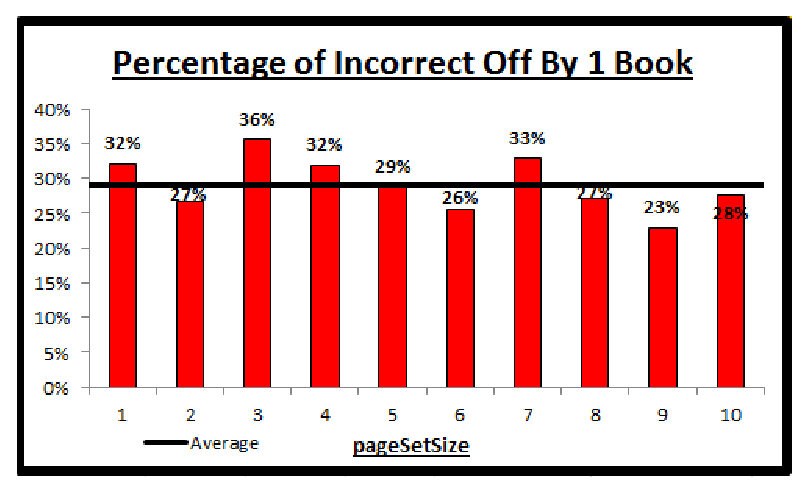
\includegraphics{naive_bayes/Images/offBy1}

Interestingly however, it seems from the confusion matrices that book
6 in particular is easily confused with and thus very similar to books
5 and 7.

\subsection{Conclusion}

\section{k-Means Clustering}

\subsection{Background}

``K-means clustering is a type of unsupervised learning, which is
used when you have unlabeled data (i.e., data without defined categories
or groups). The goal of this algorithm is to find groups in the data,
with the number of groups represented by the variable K. The algorithm
works iteratively to assign each data point to one of K groups based
on the features that are provided. Data points are clustered based
on feature similarity. The results of the K-means clustering algorithm
are:
\begin{itemize}
\item The centroids of the K clusters, which can be used to label new data
\item Labels for the training data (each data point is assigned to a single
cluster)
\end{itemize}
Rather than defining groups before looking at the data, clustering
allows you to find and analyze the groups that have formed organically.''

- Andrea Trevino (https://www.datascience.com/blog/k-means-clustering)

\subsection{Methods}

\subsubsection{Data Processing }

All the books we use are formatted to simple text files, with all
the sentences directly after each other in a single line with pages
being split up using new lines. Each book is read in separately, and
a dictionary of the words in the book is compiled, with each word
having a value of the amount of times it appeared in the book. We
chose to make all of the words lower case, in order to prevent the
same word appearing different when it was at the beginning of a sentence
or not. We also treated the different punctuation characters as separate
words. We then normalize the dictionaries by dividing the value of
each word by the total amount of words in the book the dictionary
represents (including duplicates of words in the book). This is done
in order to not bias the data towards larger books. \\
\\
After normalizing in all of the books and creating dictionaries we
sift through the dictionaries and keep only the words that appear
only in any single book. Within those words we also have a threshold
of how common the word is (how big its value is) and only keep words
whos values are above the threshold. We keep the option to remove
words as a hyper-parameter and experiment with and without removing
(see section \ref{subsec:kmeans-Hyper-Perameter-Tuning}).\\
\\
We then took the books and merged the books pages together so that
multiple pages would appear as a single page. This created books with
fewer, longer, pages. The amount of pages we merged together was kept
as a hyper-parameter we fine-tuned between different attempts (see
section \ref{subsec:kmeans-Hyper-Perameter-Tuning}). After having
our newly formatted books we took each page within each book and gave
it a value within a world consisting of a dimension for each word
that was left. The amount of dimensions in the world, which we will
reference as N, relies on the words left after removing words, and
as such relies on the threshold for removal of words, but is generally
very large. Thus the value of a page was an N-tuple given by the amount
of times a word represented by a dimension appeared in the page divided
by the amount of words in the book. 

\textbf{Note:} The normalization we applied to the dictionaries is
not applicable to a page per page basis as a single page doesn't necessarily
consist all of the appearance of a single word, thus we needed to
normalize them separately and that is the reason for the division
by the amount of words of the book of the page being given a value.\\
\\
These final page values were used as points for the k-means algorithm
to try to cluster.

\subsubsection{k-Means Procedure}

The ``k'' in k-Means represents the amount of clusters we attempted
to cluster our data to. This value was kept as a hyper-parameter and
was fine-tuned between different attempts (see section \ref{subsec:kmeans-Hyper-Perameter-Tuning}).\\

The first thing we needed to do when starting the k-Means procedure
was to randomize the centers of the initial clusters. With our first
attempts we randomized the centers generally in the Nth dimensional
world, where in each dimension it was located between the minimum
value given to any page on that dimension and the maximum value any
page was given on that dimension. This produced a lot of centers that
were centered in places where no pages were allocated for them, and
there clusters were empty. Though this remained a problem throughout
we managed to mitigate it to an extent by initializing the center
points more in the middle of the world. This was done by randomizing
the location of each center in each dimension within an interval around
the average of values of the pages in that dimension.\\

After initializing the centers we performed the following k-Means
algorithm:

\begin{algorithm}

\caption{k-Means}

\begin{lstlisting}
Initialize clusters to be empty
While(clusters have changed in last itteration):
	For each page:
		Check which cluster center is closest to page and assign it to that cluster
	
	For each cluster center:
		Find the average of all the points in the cluster and set cluster center to it.
\end{lstlisting}
\end{algorithm}

We printed out the amount of pages from each book in each cluster
and followed that to see if any interesting patterns emerged.

\subsubsection{Hyper-Parameter Tuning\label{subsec:kmeans-Hyper-Perameter-Tuning}}

The hyper-parameters that we tuned between runs were:
\begin{itemize}
\item Amount of pages to be merged when reformatting the books
\item k - the amount of clusters to use
\item Whether to remove words
\item The threshold for removing words
\end{itemize}

\paragraph{}

\subsection{Results}

\subsubsection{Confusion Matrix}

\subsection{Conclusion}
\end{document}
